\documentclass[a4paper,8pt]{report}

\usepackage[francais]{babel}
\usepackage[T1]{fontenc}
\usepackage[latin1]{inputenc}

\usepackage[left=2cm]{geometry}
\usepackage{amsmath,amssymb,mathrsfs}
\usepackage{graphicx}

%Utilisation des codes sources en C
\usepackage{listings}
\lstset{
  language=C,
  language=Bash,
  basicstyle=\footnotesize,
  numbers=left,
  numberstyle=\normalsize,
  numbersep=7pt,
}

%titre pdf
\title{{\LARGE Algorithmique Avanc\'ee \\ Devoir de Programmation : Tries}}
\author{Bielle Benjamin - 2900825}

\graphicspath{{graph/}} 

\begin{document}

\maketitle
\renewcommand{\contentsname}{Sommaire}
\tableofcontents

\chapter{Structures}
\section*{Arbres de la Briandais}\label{sec:name}
\addcontentsline{toc}{section}{Arbres de la Briandais}

Parmi le code ASCII nous pouvons d\'eterminer plusieurs marqeurs de fin de chain (ou de fin d'un mot).\\
Par exemple, les carat\`eres '*' ou '\#' mais ici nous prendrons le caract\`ere '\textbackslash0' le marqueur de fin de chaine ainsi la programmation de notre projet en sera facilit\'ee.

\medskip
Pour nous aider dans la construction d'un arbre de la Briandais, nous allons utiliser des primitives de base :\\
\begin{itemize}
\item newBRDtree (cl\'e : Mot, fils : BRDtree, fr\`ere : BRDtree).\\
  $\rightarrow$ retourne un arbre de la Briandais (BRDtree).\\
\item buildBRDtree (m : Mot).\\
  $\rightarrow$ retourne un arbre de la Briandais construit \`a partir du mot m (BRDtree).\\
\item addBRDtree (m : Mot, Tree : BRDtree).\\
  $\rightarrow$ ajoute un mot \`a un arbre de la Briandais (BRDtree).\\
\item emptyBRDtree ().\\
  $\rightarrow$ retourne un arbre de la Briandais vide.\\
\item isEmpty (arbre : BRDtree).\\
  $\rightarrow$ test si l'arbre est vide.\\
\item head (m : Mot).\\
  $\rightarrow$ retourne la premi\`ere lettre du mot m.\\
\item tail (m : Mot).\\
  $\rightarrow$ idem \`a la fonction head, retourne le reste des lettres du mot m (tout sauf la premi\`re lettre).\\
\end{itemize}

Nous allons construire un arbre de la Briandais \`a partir du texte \textbf{exemple de base}:\\
\textit{"A quel genial professeur de dactylographie sommes nous redevables de la superbe phrase ci dessous, un modele du genre, que toute dactylo connait par coeur puisque elle fait appel a chacune des touches du clavier de la machine a ecrire ?"}

\begin{figure}[H]
  \centering
  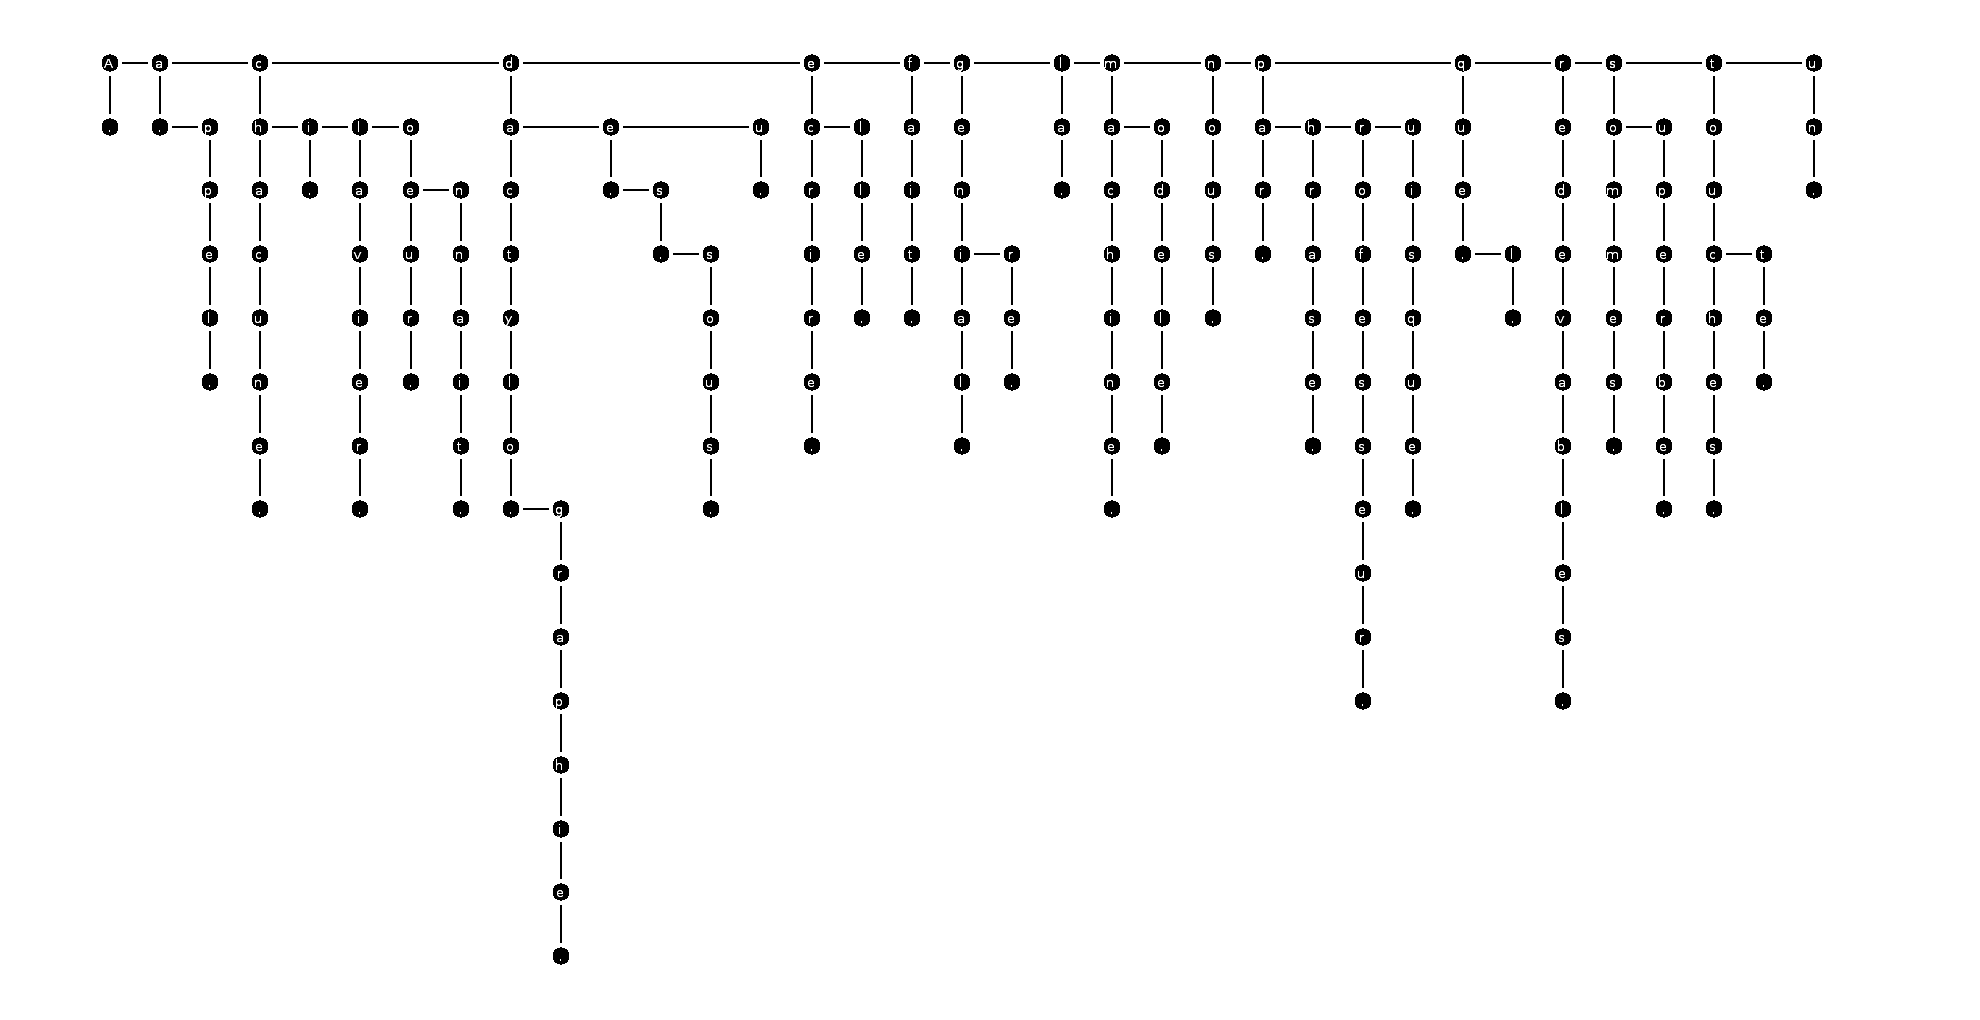
\includegraphics[width=0.8\textwidth]{briandais.png}
  \caption{Arbre de la Briandais}
  \label{fig:Arbre de la Briandais}
\end{figure}
\medskip
Pour avoir une image plus graphique de cet arbre, veuillez voir la figure \ref{fig:Arbre de la Briandais} page~\pageref{fig:Arbre de la Briandais}

\section*{Tries Hybrides}\label{sec:name}
\addcontentsline{toc}{section}{Tries Hybrides}

Comme pour l'arbre de la Briandais, nous allons d\'efinir des primitives nous permettant de constuire notre trie hybride :\\
\begin{itemize}
\item Hybrid (cl\'e : Mot, valeur : Mot, inf\'erieur : THybrid, sup\'erieur : THybrid, \'egale : THybrid).\\
  $\rightarrow$ retourne un trie hybride (THybrid).\\
\item emptyTHybrid ().\\
  $\rightarrow$ retourne un trie hybride vide.\\
\item isEmpty (trie : THybrid).\\
  $\rightarrow$ test si le trie est vide.\\
\item buildTHybrid (m : Mot).\\
  $\rightarrow$ retourne le trie hybride du mot m.\\
\item addTHybrid (m : Mot, t : THybrid).\\
  $\rightarrow$ ajoute le mot m au trie hybride t.\\
\end{itemize}

Idem \`a la premi\`ere partie (arbre de la Briandais), nous allons construire un trie hybride \`a partir du texte \textbf{exemple de base}:\\
\begin{figure}[H]
  \centering
  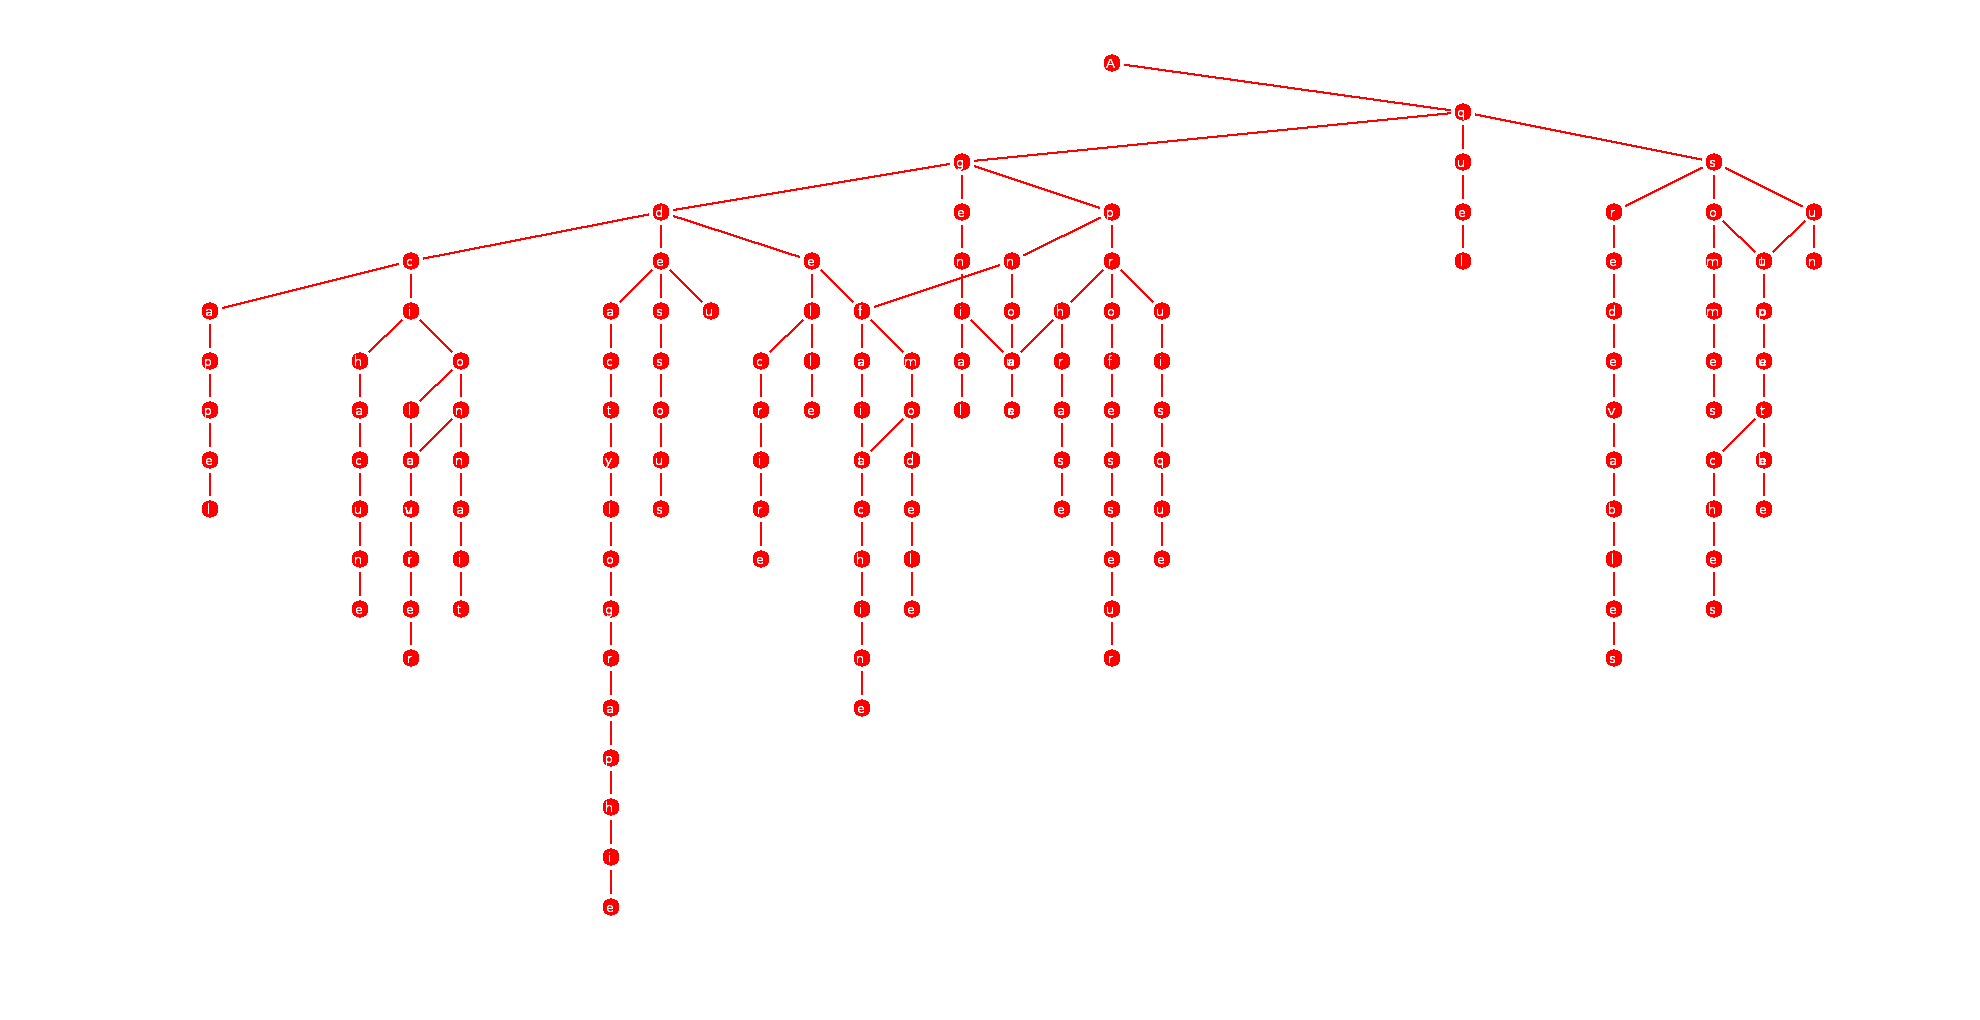
\includegraphics[width=0.8\textwidth]{hybrid.png}
  \caption{Trie Hybride}
  \label{fig:Trie Hybride}
\end{figure}
\medskip
Pour avoir une image plus graphique de ce trie, veuillez voir la figure \ref{fig:Trie Hybride} page~\pageref{fig:Trie Hybride}

\chapter{Fonctions avanc\'ees pour chacune des structures}

\section*{Fonctions pour un arbre de la Briandais}\label{sec:name}
\addcontentsline{toc}{section}{Fonctions pour un arbre de la Briandais}

fonction de recherche d'un mot dans un dictionnaire : \textit{Recherche(arbre,mot) $\rightarrow$ bool\'een}.
\begin{verbatim}
  int searchBRDtree(char *word, BRDtree *Tree)
  {
    if(strcmp(word, "") == 0)
    {
      return isEmpty(T);
    }
    else if(isEmpty(T)) return FALSE;
    if(head(word) < T->key) return FALSE;
    else if(head(word) == T->key) return searchBRDtree(tail(word), T->child);
    else return searchBRDtree(word, T->next);
  }
\end{verbatim}

fonction qui compte les mots pr\'esents dans le dictionnaire : \textit{ComptageMots(arbre) $\rightarrow$ entier}.
\begin{verbatim}
  int countWordsBRDtree(BRDtree *Tree)
  {
    if(Tree == NULL)
       return 0;
    if(Tree->key == '\0')
       return 1 + countWordsBRDtree(Tree->next);

    return countWordsBRDtree(Tree->child) + countWordsBRDtree(Tree->next);
  }
\end{verbatim}

fonction qui liste les mots du dictionnaire dans l'ordre alphab\'etique : \textit{ListeMots(arbre) $\rightarrow$ liste[mots]}.
\begin{verbatim}
  void addWordList(char *word, wordList **list)
  {
     wordList *new = (wordList *) malloc(sizeof(wordList));
     new->word = word;
     new->next = *list;
     *list = new;
  }

  void insideListWordsBRDtree(BRDtree *Tree, wordList **list, char *word)
  {
     if(Tree == NULL)
        return;
     int n = strlen(word);
     char *newWord = (char *) malloc(sizeof(char) * (n + 1));
     int i;
     for(i = 0; i < n; i++)
         newWord[i] = word[i];
     newWord[i] = Tree->key;
     if(Tree->key == '\0')
         addWordList(newWord, list);
     insideListWordsBRDtree(Tree->child, list, newWord);
     insideListWordsBRDtree(Tree->next, list, word);
  }

  wordList *listWordsBRDtree(BRDtree *Tree)
  {
     wordList *list = (wordList *) malloc(sizeof(wordList));
     list->word = "";        
     list->next = NULL;
     insideListWordsBRDtree(Tree, &list, "");
     
     return list;
  }
\end{verbatim}

fonction qui compte les pointeurs vers NIL : \textit{ComptageNil(arbre) $\rightarrow$ entier}.
\begin{verbatim}
  int countNullBRDtree(BRDtree *Tree)
  {
    if(Tree == NULL)
       return 1;
    if(isEmpty(Tree))
       return 2;
    return countNullBRDtree(Tree->child) + countNullBRDtree(Tree->next);
  }
\end{verbatim}

fonction qui calcule la hauteur de l'arbre : \textit{Hauteur(arbre) $\rightarrow$ entier}.
\begin{verbatim}
  int heightBRDtree(BRDtree *Tree)
  {
     if(isEmpty(Tree)) return 0;
     return max(1 + heightBRDtree(Tree->child), heightBRDtree(Tree->next));
  }
\end{verbatim}

fonction qui calcule la profondeur moyenne des feuilles de l'arbre : \textit{ProfondeurMoyenne(arbre) $\rightarrow$ entier}.
\begin{verbatim}
  void insideAverage(BRDtree *Tree, int *level, int *count, int currLevel)
  {
    if(Tree == NULL) return;
    (*level) += currLevel;
    (*count)++;
    if(Tree->child != NULL)
       insideAverage(Tree->child, level, count, currLevel + 1);
    if(Tree->next != NULL)
       insideAverage(Tree->next, level, count, currLevel);
  }

  double averageLevelBRDtree(BRDtree *Tree)
  {
    int  level = 0, count = 0, currLevel = 1;
    insideAverage(Tree, &level, &count, currLevel);
    if(count == 0) return 0.0;
    return (double) level / count;
  }
\end{verbatim}

fonction qui prend un mot A en argument et qui indique de combien de mots du dictionnaire le mot A est le pr\'efixe : \textit{Prefixe(arbre,mot) $\rightarrow$ entier}.
\begin{verbatim}
  int countPrefixBRDtree(char *prefix, BRDtree *Tree)
  {
     if(strcmp(prefix, "") == 0)
        return countWordsBRDtree(Tree);
     if(head(prefix) < Tree->key)
        return 0;
     else if (head(prefix) > Tree->key)
        return countPrefixBRDtree(prefix, Tree->next);
     else
        return countPrefixBRDtree(tail(prefix), Tree->child);
  }
\end{verbatim}

fonction qui prend un mot en argument et qui le supprime de l'arbre \textbf{s'il y figure} : \textit{Suppression(arbre,mot) $\rightarrow$ arbre}.
\begin{verbatim}
  BRDtree *delBRDtree(char *word, BRDtree *Tree)
  {
     if(Tree == NULL)
        return NULL;
     if(isEmpty(Tree) && strcmp(word, "") == 0)
        return Tree->next;
     if(Tree->key == head(word))
     {
        BRDtree *child = delBRDtree(tail(word), Tree->child);
        if(child == NULL)
            return Tree->next;
        else
            return BRD(Tree->key, child, Tree->next);
     }
     else if(Tree->key > head(word))
        return Tree;
     else
        return BRD(Tree->key, Tree->child, delBRDtree(word, Tree->next));
  }
\end{verbatim}

\section*{Fonctions pour un trie hybride}\label{sec:name}
\addcontentsline{toc}{section}{Fonctions pour un trie hybride}

fonction de recherche d'un mot dans un dictionnaire : \textit{Recherche(arbre,mot) $\rightarrow$ bool\'een}.\textbf{\`a faire}
\begin{verbatim}
\end{verbatim}

fonction qui compte les mots pr\'esents dans le dictionnaire : \textit{ComptageMots(arbre) $\rightarrow$ entier}.\textbf{\`a faire}
\begin{verbatim}
\end{verbatim}

fonction qui liste les mots du dictionnaire dans l'ordre alphab\'etique : \textit{ListeMots(arbre) $\rightarrow$ liste[mots]}.\textbf{\`a faire}
\begin{verbatim}
\end{verbatim}

fonction qui compte les pointeurs vers NIL : \textit{ComptageNil(arbre) $\rightarrow$ entier}.\textbf{\`a faire}
\begin{verbatim}
\end{verbatim}

fonction qui calcule la hauteur de l'arbre : \textit{Hauteur(arbre) $\rightarrow$ entier}.\textbf{\`a faire}
\begin{verbatim}
\end{verbatim}

fonction qui calcule la profondeur moyenne des feuilles de l'arbre : \textit{ProfondeurMoyenne(arbre) $\rightarrow$ entier}.\textbf{\`a faire}
\begin{verbatim}
\end{verbatim}

fonction qui prend un mot A en argument et qui indique de combien de mots du dictionnaire le mot A est le pr\'efixe : \textit{Prefixe(arbre,mot) $\rightarrow$ entier}.\textbf{\`a faire}
\begin{verbatim}
\end{verbatim}

fonction qui prend un mot en argument et qui le supprime de l'arbre \textbf{s'il y figure} : \textit{Suppression(arbre,mot) $\rightarrow$ arbre}.\textbf{\`a faire}
\begin{verbatim}
\end{verbatim}

\chapter{Fonctions complexes}

\chapter{Complexit\'es}

\chapter{Annexe}
\section*{Structures de donn\'ees}\label{sec:name}
\addcontentsline{toc}{section}{Structures de donn\'ees}

Ici nous d\'etaillerons les diff\'erentes structures de donn\'ees utilis\'ees dans ce projet.

\subsection*{Arbres de la Briandais}\label{sec:name}
\addcontentsline{toc}{subsection}{Arbres de la Briandais}

La structure de donn\'ees \textit{BRDtree} est la structure d\'efinissant un arbre de la Briandais.
\begin{verbatim}
  typedef struct BRDtree
  {
     char key; 
     struct BRDtree *child; 
     struct BRDtree *next; 
  }BRDtree;
\end{verbatim}

La structure de donn\'ees \textit{wordList} est la structure d\'efinissant une liste de mots pour un arbre de la Briandais.
\begin{verbatim}
  typedef struct wordList
  {
     char *word;
     struct wordList *next;
  }wordList;
\end{verbatim}

\subsection*{Tries Hybrides}\label{sec:name}
\addcontentsline{toc}{subsection}{Tries Hybrides}

La structure de donn\'ees \textit{THybrid} est la structure d\'efinissant un trie hybride.
\begin{verbatim}
  typedef struct THybrid
  {
     char key;
     char val;
     struct THybrid *inf;
     struct THybrid *eq;
     struct THybrid *sup;
  }THybrid;
\end{verbatim}

\addcontentsline{toc}{section}{\listfigurename}
\listoffigures
\newpage
\section*{Bibliographie}\label{sec:name}
\addcontentsline{toc}{section}{Bibliographie}

\end{document}
